%%%%%%%%%%%%%%%%%%%%%%%%%%%%%%%%%%%%%%%%%
% baposter Portrait Poster
% LaTeX Template
% Version 1.0 (15/5/13)
%
% Created by:
% Brian Amberg (baposter@brian-amberg.de)
%
% This template has been downloaded from:
% http://www.LaTeXTemplates.com
%
% License:
% CC BY-NC-SA 3.0 (http://creativecommons.org/licenses/by-nc-sa/3.0/)
%
%%%%%%%%%%%%%%%%%%%%%%%%%%%%%%%%%%%%%%%%%

%----------------------------------------------------------------------------
%	PACKAGES AND OTHER DOCUMENT CONFIGURATIONS
%----------------------------------------------------------------------------

\documentclass[a0paper,portrait,fontscale=0.395]{baposter}

\usepackage[font=small,labelfont=bf]{caption} % Required for specifying captions to tables and figures
\usepackage{booktabs} % Horizontal rules in tables
\usepackage{enumitem} % To change spacing in itemize and enumerate lists
\usepackage{multicol}
\usepackage{relsize} % Used for making text smaller in some places
\usepackage{amsfonts, amsmath, amsthm, amssymb} % For math fonts, symbols and environments
\usepackage{wrapfig} % Allows wrapping text around tables and figures
\usepackage[export]{adjustbox}% http://ctan.org/pkg/adjustbox
\usepackage{palatino} % Uncomment to use the Palatino font
\usepackage{graphicx} % Required for including images
\usepackage{color}
\usepackage{mathtools}
\usepackage{svg}

\graphicspath{{figures/}} % Directory in which figures are stored

\definecolor{bordercol}{RGB}{256,256,256} % Border color of content boxes
\definecolor{headercol1}{RGB}{51,0,111} % Background color for the header in the content boxes (left side)
\definecolor{headercol2}{RGB}{51,0,111} % Background color for the header in the content boxes (right side)
\definecolor{headerfontcol}{RGB}{256,256,256} % Text color for the header text in the content boxes
\definecolor{boxcolor}{RGB}{256,256,256} % Background color for the content in the content boxes

\newenvironment{Figure}
  {\par\medskip\noindent\minipage{\linewidth}}
  {\endminipage\par\medskip}

\DeclarePairedDelimiterX{\norm}[1]{\lVert}{\rVert}{#1}
\DeclareMathOperator{\Tr}{Tr}

\begin{document}

\begin{poster}{
grid=false,
headerheight=0.075\textheight,
borderColor=bordercol, % Border color of content boxes
headerColorOne=headercol1, % Background color for the header in the content boxes (left side)
headerColorTwo=headercol2, % Background color for the header in the content boxes (right side)
headerFontColor=headerfontcol, % Text color for the header text in the content boxes
boxColorOne=boxcolor, % Background color for the content in the content boxes
headershape=roundedright, % Specify the rounded corner in the content box headers
headerfont=\Large\sf\bf, % Font modifiers for the text in the content box headers
textborder=rectangle,
background=none,
headerborder=open, % Change to closed for a line under the content box headers
boxshade=plain
}
{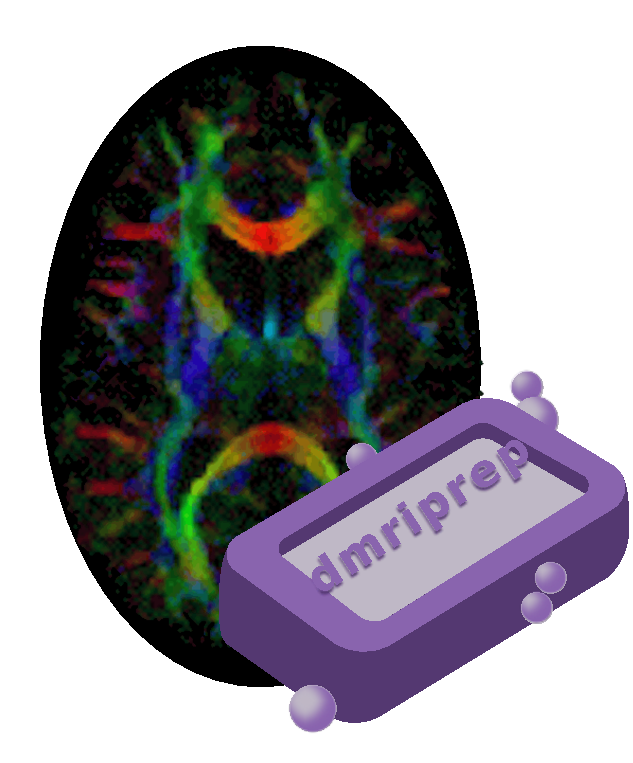
\includegraphics[scale=0.3]{dmriprep_icon.pdf}}
%
%----------------------------------------------------------------------------
%	TITLE AND AUTHOR NAME
%----------------------------------------------------------------------------
%
{\sf\bf DMRIprep: a Robust, Scalable Preprocessing \\ Pipeline for diffusion MRI} % Poster title
{\vspace{0.3em}\hspace{0.5em} Adam Richie-Halford\textsuperscript{1}, Jason Yeatman\textsuperscript{2}, Ariel Rokem\textsuperscript{1}, Anisha Keshavan\textsuperscript{3} \hfill Poster W624 \hspace{0.5em}\null \\ % Author names
{\hspace{0.65em}\smaller 1. University of Washington, 2. Stanford University, 3. Child Mind Institute \hfill Contact: richford@uw.edu \hspace{0.5em}\null}} % Author email addresses
{
\includegraphics[scale=0.12]{UWlogo.png}} % University/lab logo

%----------------------------------------------------------------------------
%	INTRODUCTION
%----------------------------------------------------------------------------

\headerbox{Introduction}{name=introduction,column=0,row=0}{

\noindent Diffusion MRI (dMRI) is the only existing method to analyze human white matter \emph{in vivo}, but requires a pipeline of steps to preprocess the data, e.g.
\begin{itemize}[noitemsep]
    \item eddy current correction,
    \item motion correction,
    \item gradient direction adjustment.
\end{itemize}
\textbf{\underline{Challenge}: Complexity and lack of standardization of preprocessing can induce bias in interpretation of dMRI.}
\begin{Figure}
    \centering
    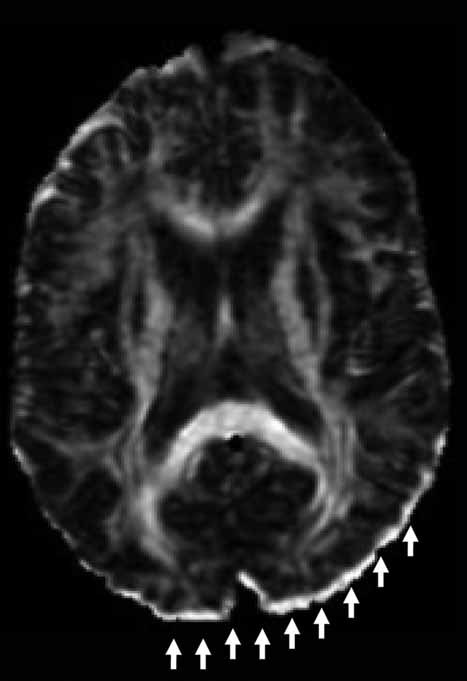
\includegraphics[height=0.45\linewidth, frame]{pitfalls_eddy_current.jpg}
    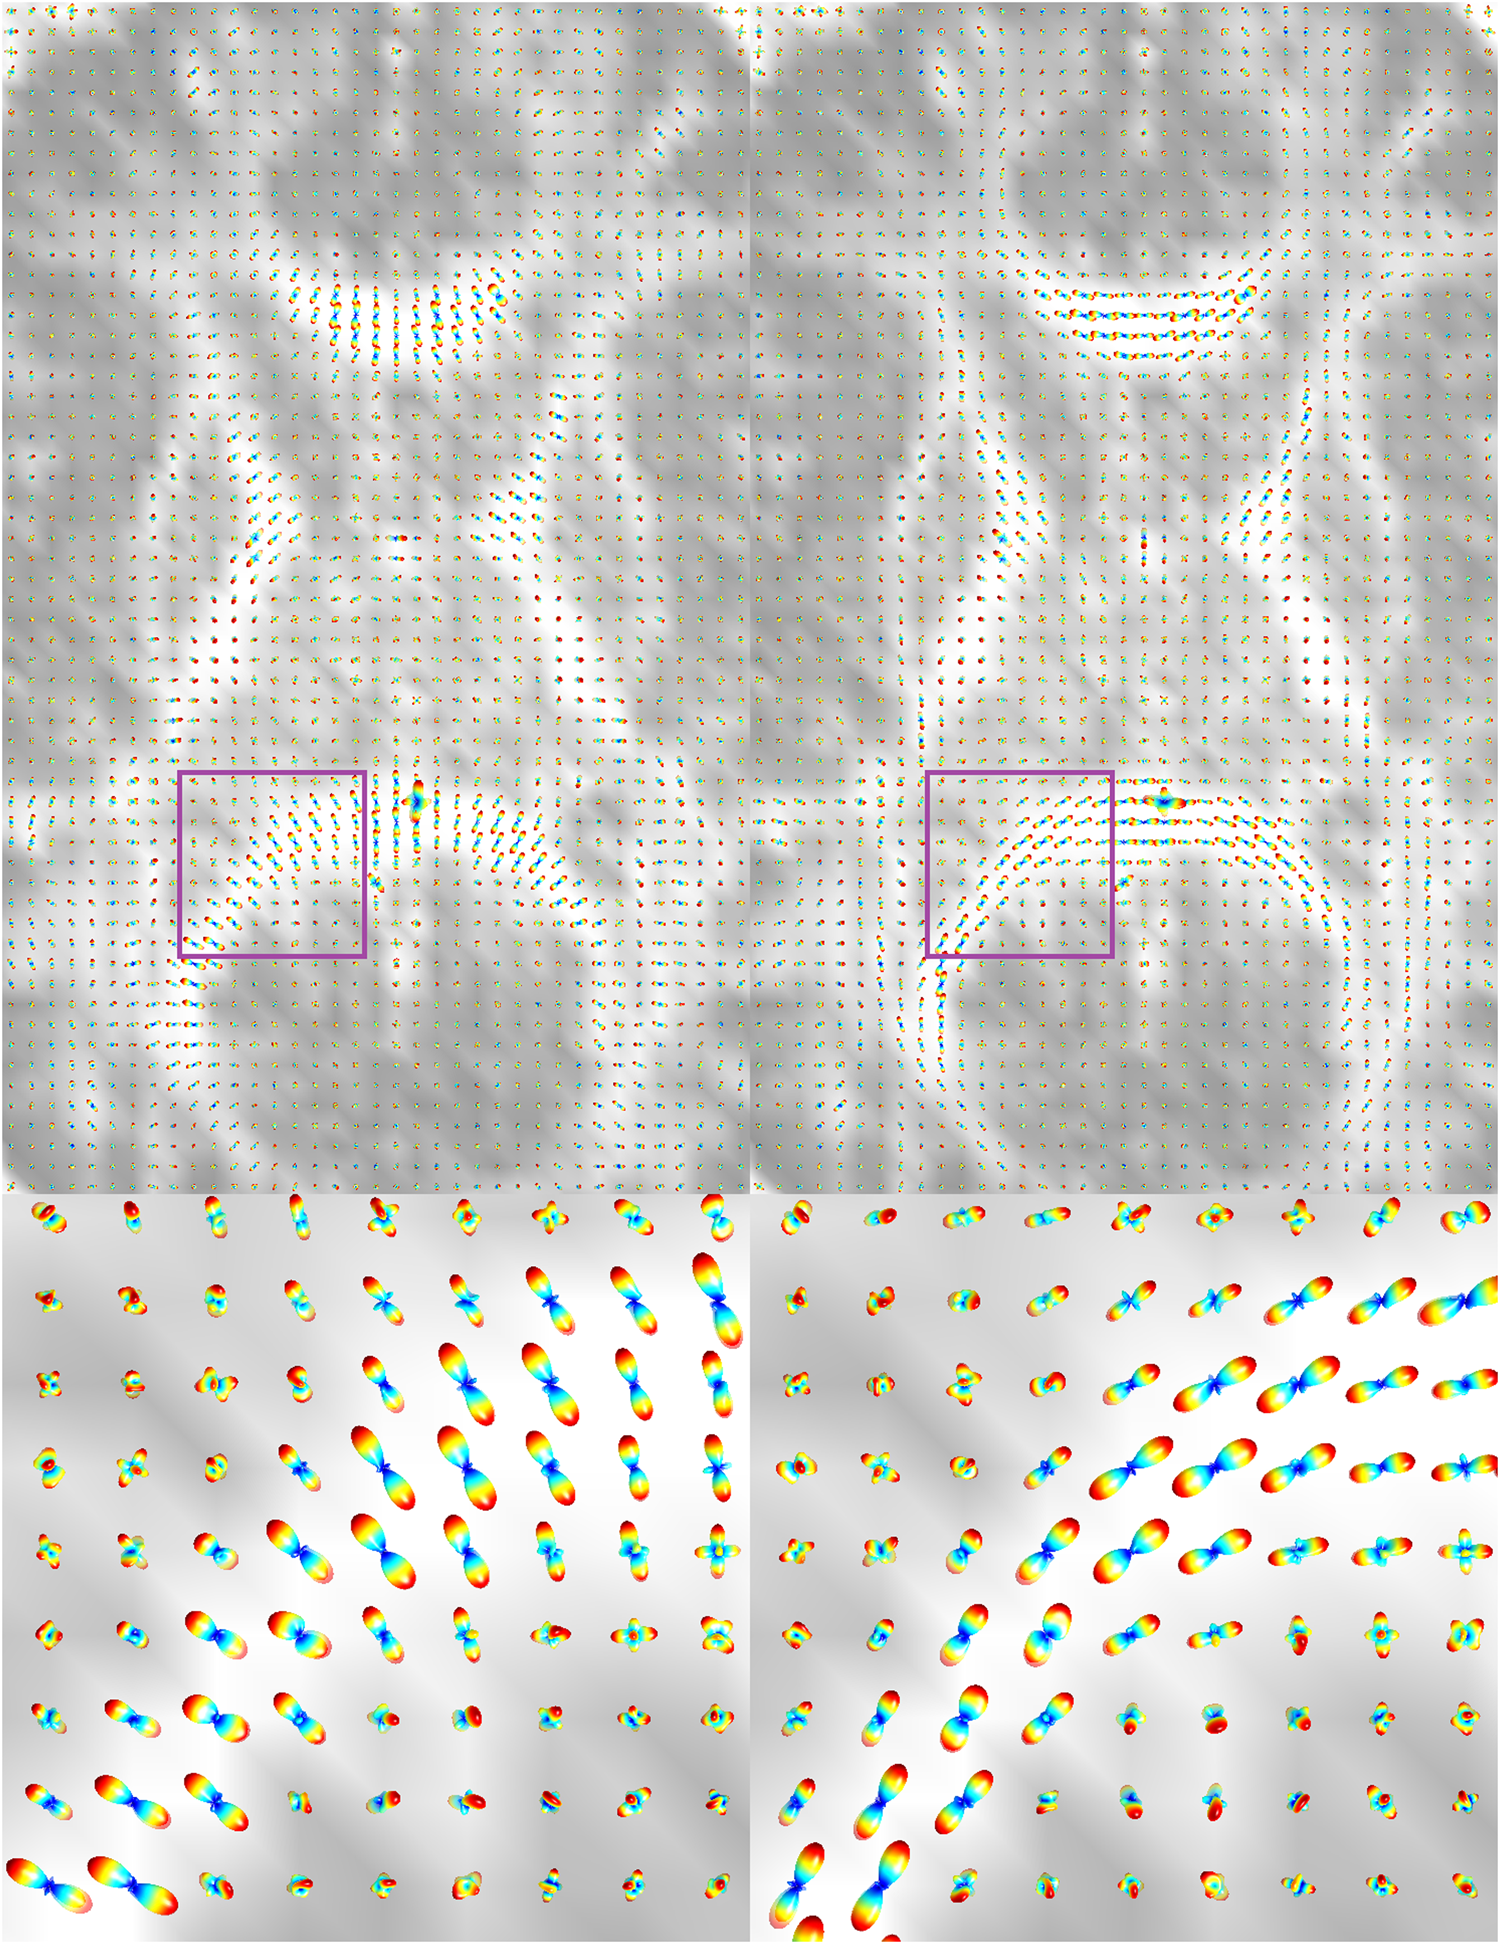
\includegraphics[height=0.45\linewidth, frame]{pitfalls_axis_flip.png}
    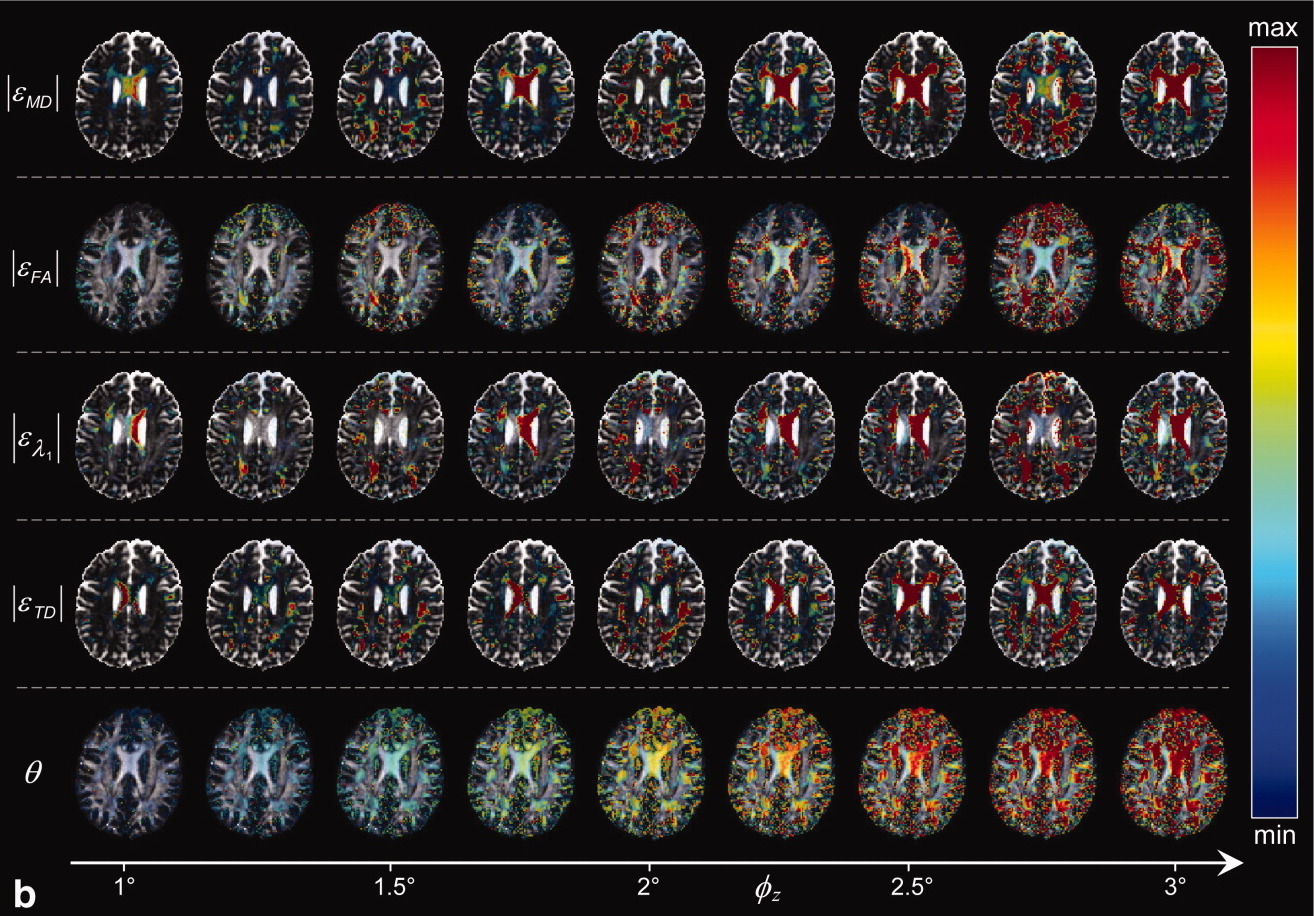
\includegraphics[width=0.7\linewidth, frame]{pitfalls_orient_bvector.jpg}
    \captionof{figure}{\textbf{top left}: eddy current artifacts\cite{jones2010twenty}, \textbf{top right}: consequence of gradient table flip artifact\cite{aganj2018automatic}, \textbf{bottom}: effects of not reorienting the $\mathbf{b}$-matrix when correcting for motion\cite{leemans2009b}.}
\end{Figure}

\noindent In the related field of fMRI, the FMRIprep software\cite{esteban2019fmriprep} successfully standardized preprocessing to reduce errors and increase reproducibility. Inspired by this success, DMRIprep applies the philosophy of FMRIprep to dMRI analysis. It is designed to be
\vspace{-0.5em}
\begin{multicols}{2}
\begin{itemize}[nosep]
    \item robust
    \item reproducible
    \item interrogable
    \item scalable
\end{itemize}
\end{multicols}
}

%----------------------------------------------------------------------------
%	METHODS
%----------------------------------------------------------------------------

\headerbox{Methods}{name=methods,column=0,below=introduction}{

\noindent DMRIprep is implemented as a nipype\cite{gorgolewski2016brain} workflow including:
\begin{itemize}[noitemsep, leftmargin=*]
    \item Eddy current correction using FSL.
    \item Coregistration to a T1W image with Freesurfer.
    \item Production of QC reports using EDDY QC\cite{bastiani2019automated} and DIPY\cite{garyfallidis2014dipy}.
    \item A custom interactive report website.
\end{itemize}
\vspace{-0.5em}
\begin{Figure}
    \centering
    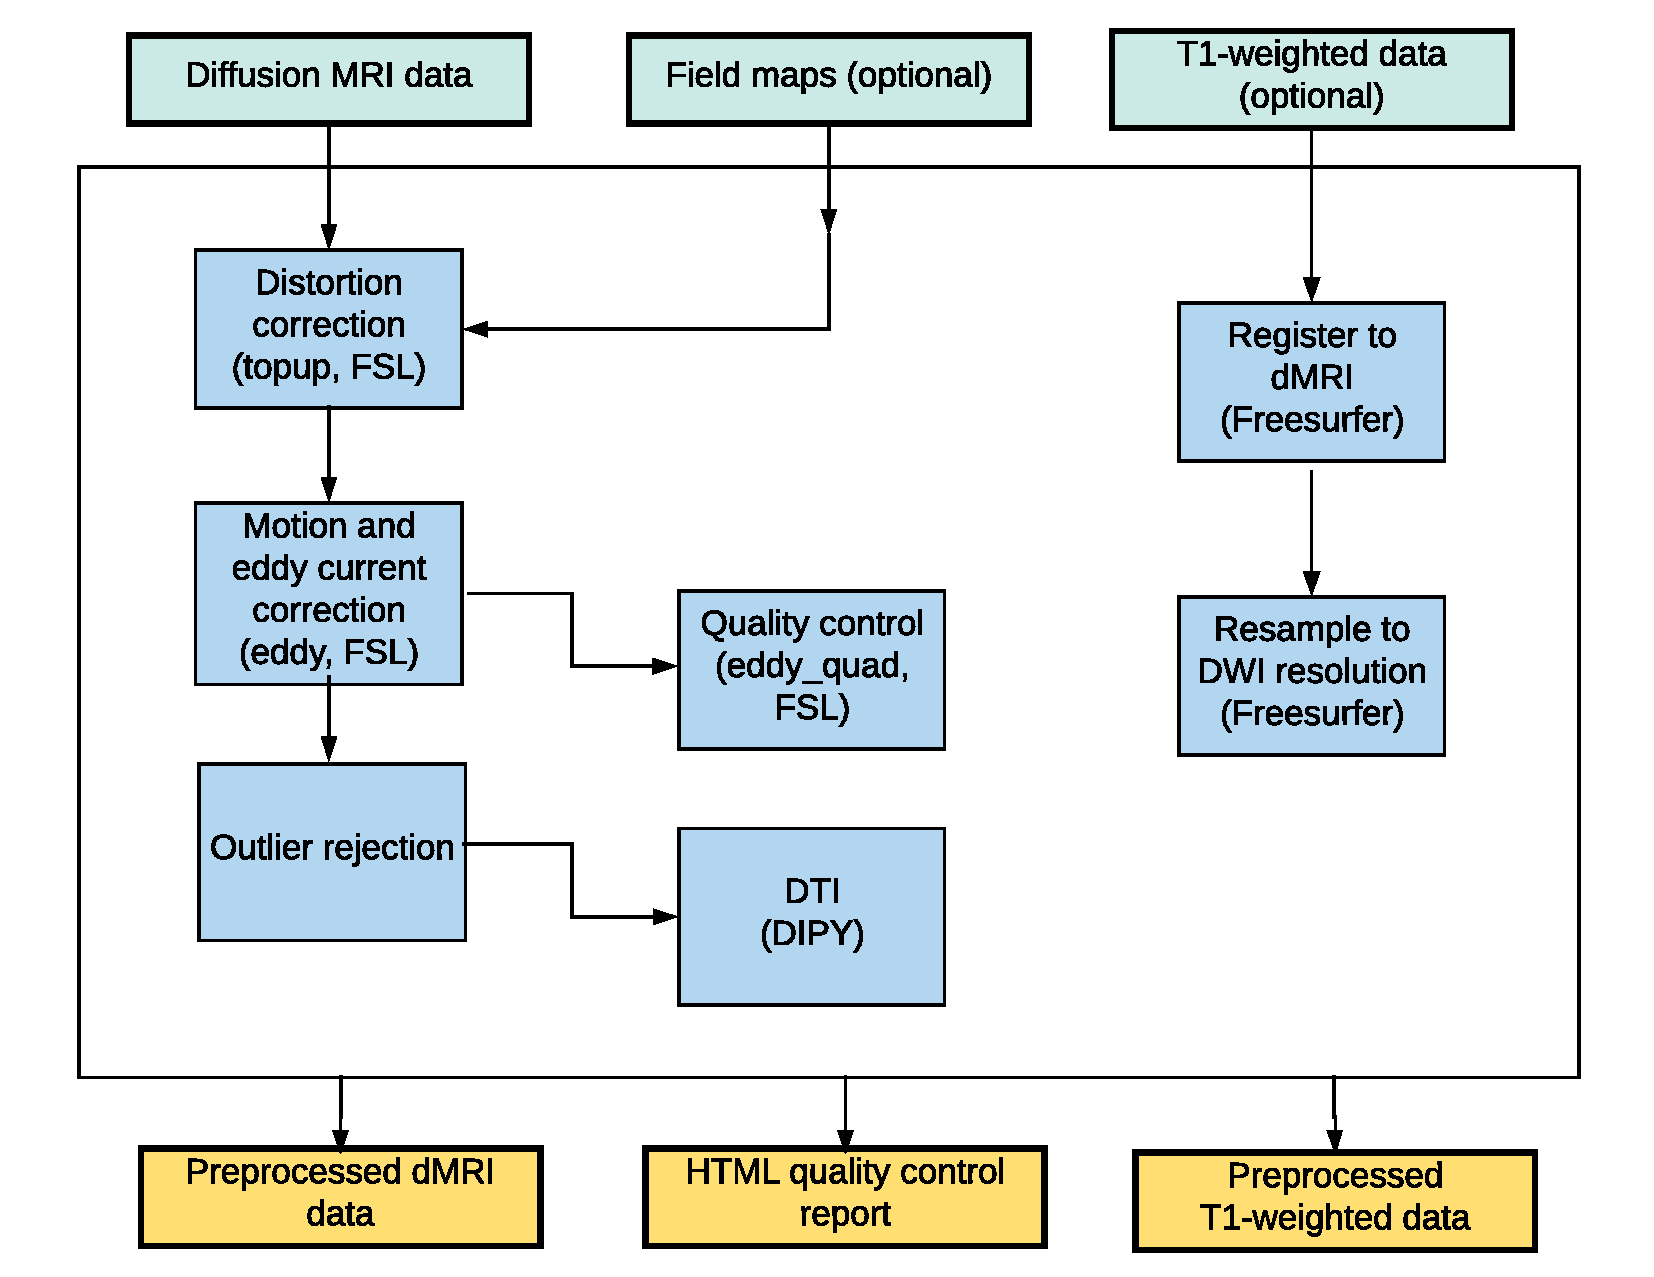
\includegraphics[width=0.82\linewidth]{dmriprep_workflow.pdf}
    \captionof{figure}{DMRIprep workflow: given input dMRI data and optional EPI field maps, FSL's \texttt{topup} and \texttt{eddy} correct for distortions, motion, and eddy currents. DMRIprep removes volumes that exceed a user-defined threshold for outlier slices. \texttt{eddy\_quad} generates QC reports, which are organized into an interactive report webpage. DIPY computes the diffusion tensor images of the corrected data. Separately, the input structural images are registered to the dMRI data and resampled to DWI resolution. Output is organized in BIDS format for further analysis.}
\end{Figure}

\noindent All DMRIprep dependencies are packaged into a Docker image with three command line tools:
\begin{itemize}[noitemsep, leftmargin=*]
    \item \texttt{dmriprep}: a BIDS-App compliant tool that runs the primary workflow,
    \item \texttt{dmriprep-data}: a tool to download data from public datasets and transform the files to BIDS-format,
    \item \texttt{dmriprep-upload}: a tool to upload DMRIprep results to an Amazon Web Services (AWS) S3 bucket.
\end{itemize}
}

%----------------------------------------------------------------------------
%	CONCLUSION
%----------------------------------------------------------------------------

\headerbox{Conclusion}{name=conclusion,column=0,below=methods,above=bottom}{

\begin{itemize}[nosep, leftmargin=*]
    \item DMRIprep implements
    \begin{itemize}[nosep, leftmargin=*]
        \item a nipype pipeline for preprocessing of dMRI data,
        \item web-based visualizations for quality control of results,
        \item a BIDS-App compliant command-line interface to download, preprocess, and upload large dMRI datasets.
    \end{itemize}

    \item Robust, scalable preprocessing pipeline for many different experimental settings.
    \item Improves consistency and reproducibility of analysis procedures and methods reporting.
    \item Open source: \texttt{https://github.com/nipy/dmriprep}
\end{itemize}
}

%----------------------------------------------------------------------------
%	RESULTS 1
%----------------------------------------------------------------------------

\headerbox{Results}{name=results1,span=2,column=1,row=0}{ % To reduce this block to 1 column width, remove 'span=2'

\noindent We tested DMRIprep by analyzing the Healthy Brain Network\cite{alexander2017open} (HBN) dataset.
\begin{itemize}[noitemsep]
    \item 60 subjects from three different sites (``Site-SI'', ``Site-RU'', ``Site-CBIC'')
    \item BIDS compliant (mostly)
    \item DMRIprep was able to accommodate slight irregularities in each site's file structure and format.
    \item Visually inspected QC results using DMRIprep-viewer (\texttt{http://nipy.org/dmriprep}).
\end{itemize}

\begin{Figure}
    \centering
    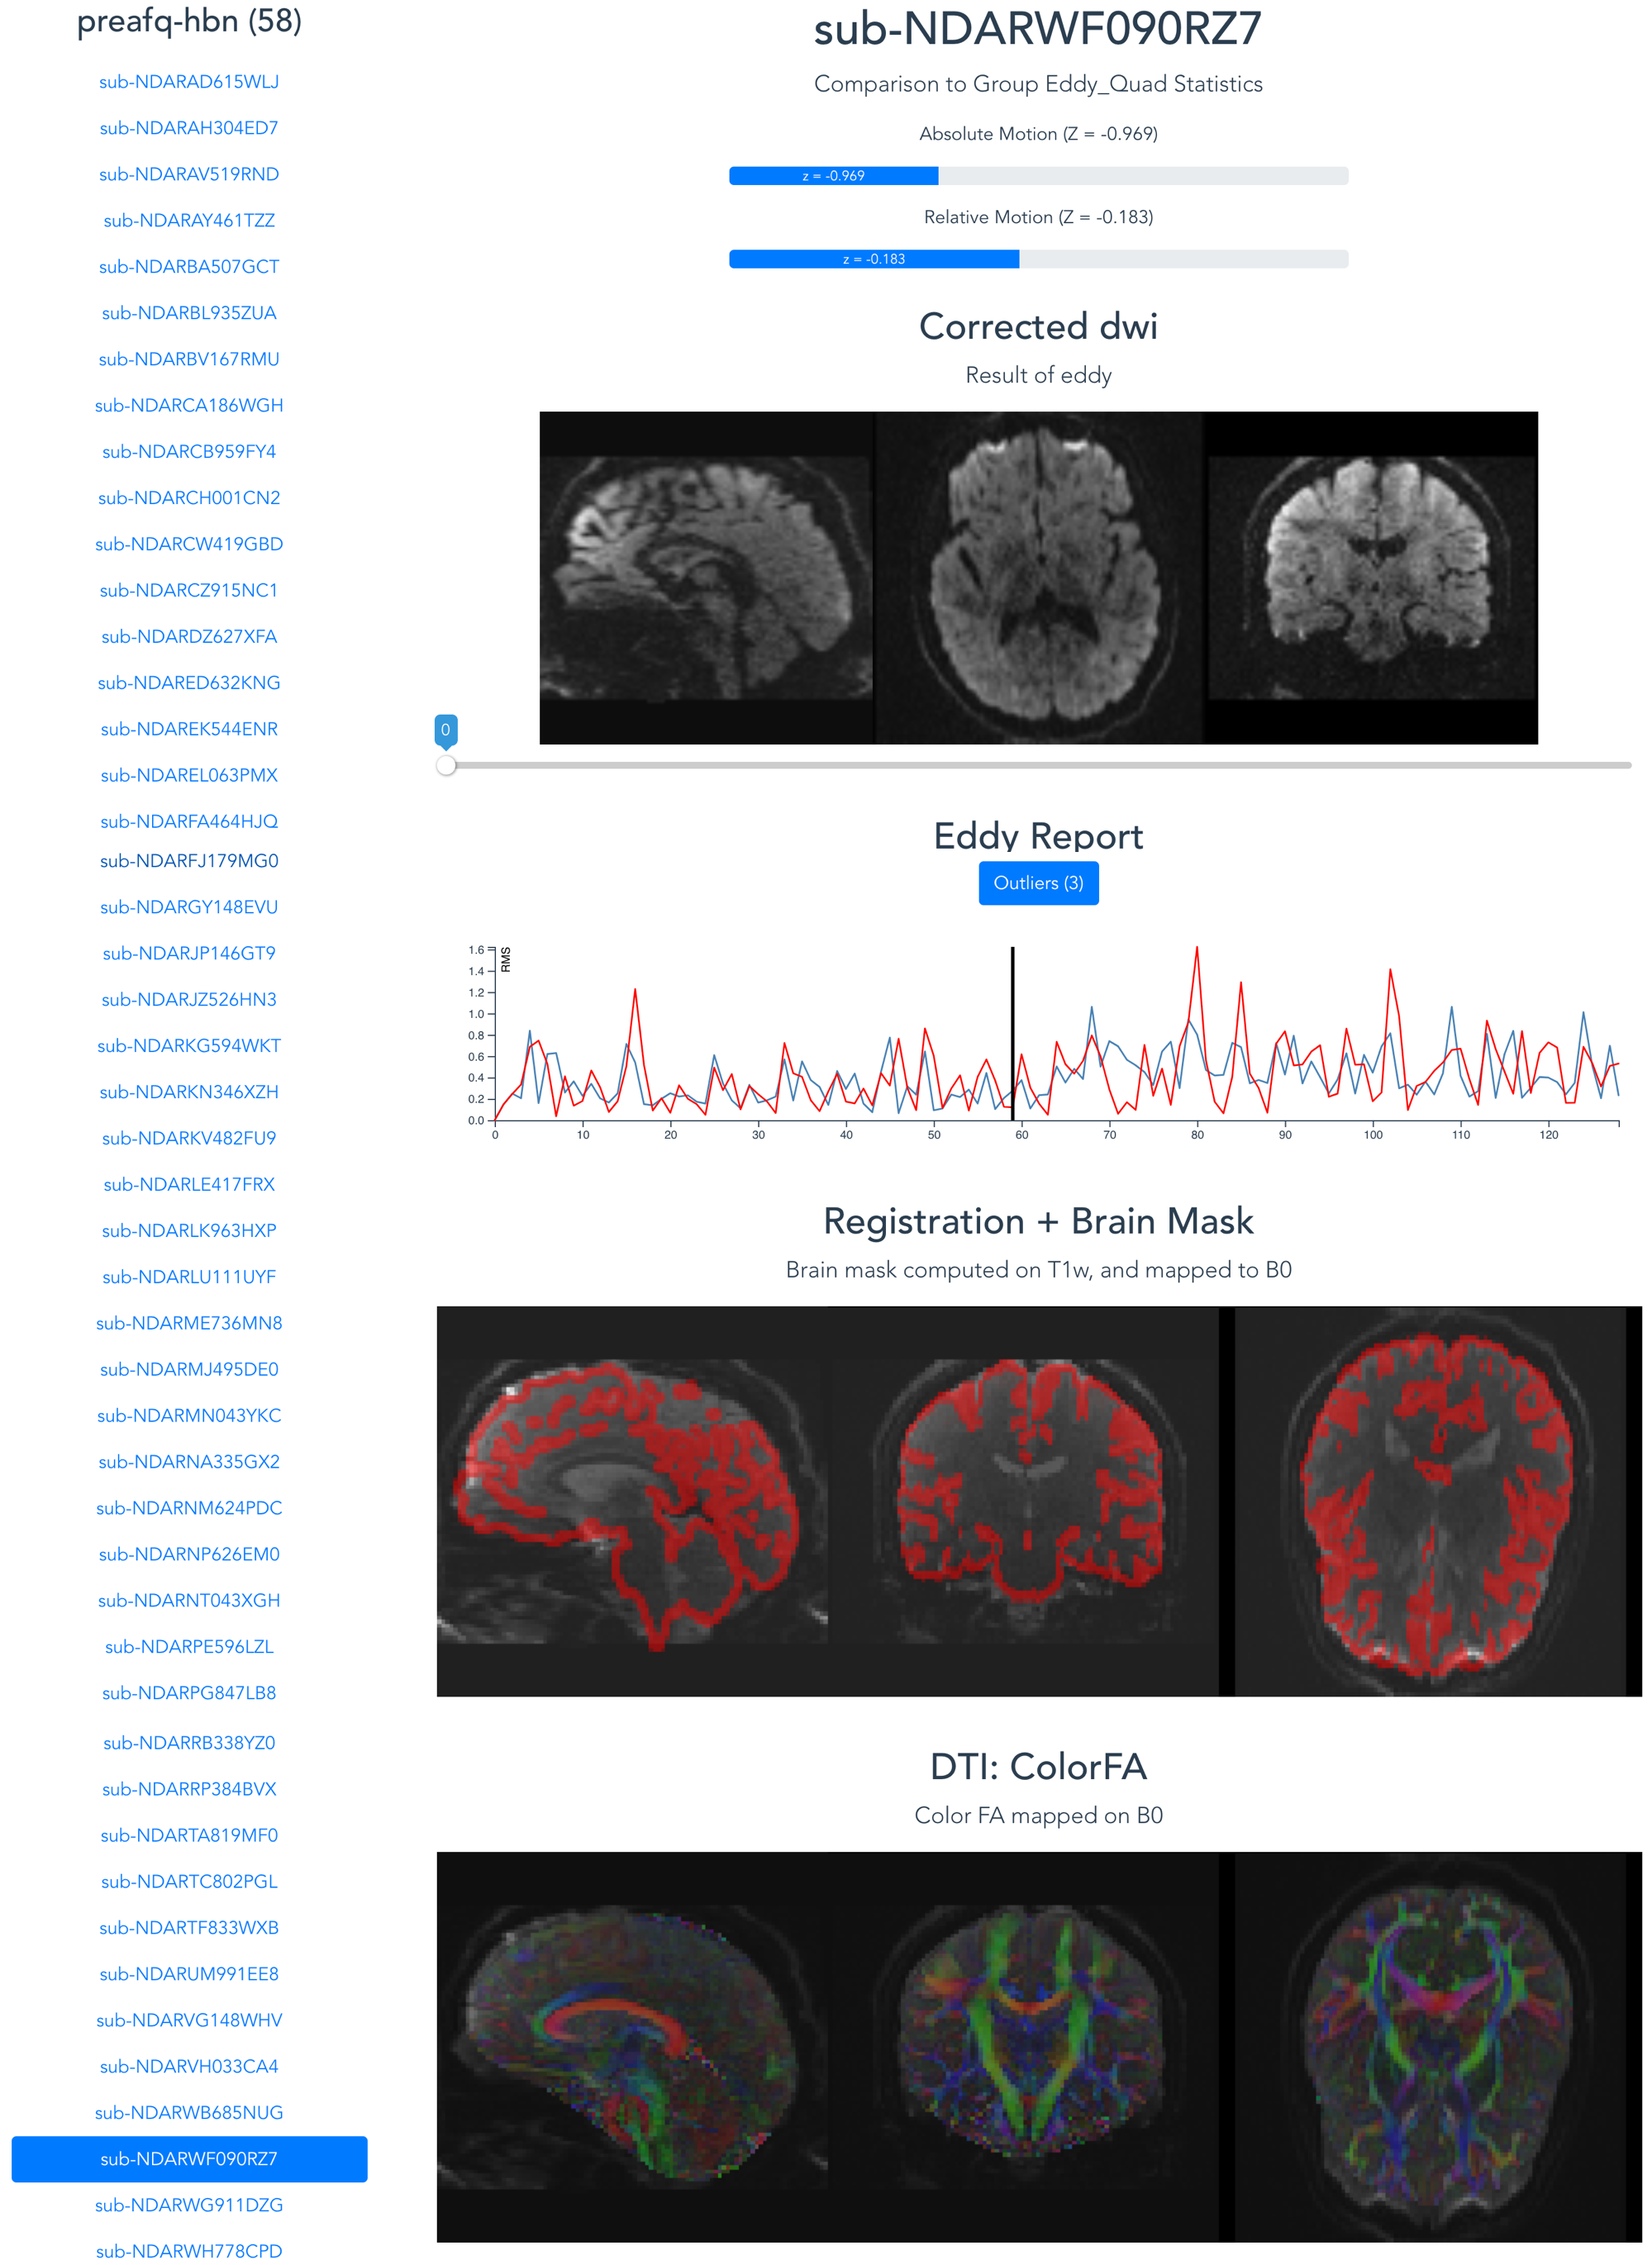
\includegraphics[width=0.87\linewidth]{qc_report.png}
    \captionof{figure}{An example DMRIprep QC report, generated with DMRIprep-viewer. From top to bottom, it displays: (1) group comparisons for relative and absolute motion; (2) a view of the eddy current-corrected DWI volumes; (3) a report of the outlier volumes and slices; (4) a view of the registration mask, mapped onto the B0 DWI images; and (5) a DTI map showing fractional anisotropy mapped onto the B0 image.}
\end{Figure}

\begin{minipage}[c]{0.6\linewidth}
\begin{itemize}[noitemsep]
    \item Preprocessing failed gracefully on two of the 60 subjects due to data acquisition errors (the b-values and b-vectors did not match the total number of volumes in the image).
    \item Running 60 subjects on Google Cloud Platform (GCP) using Kubernetes cost 51~USD in total, approximately 0.85~USD per subject (using an n1-highmem-4 machine with 26 GB of RAM and 4 vCPUs).
\end{itemize}
\end{minipage}
\begin{minipage}[c]{0.4\linewidth}
    \centering
    \null\hfill
    \begin{minipage}[t]{0.285\linewidth}
    \centering
    
\includegraphics[height=\linewidth, valign=c]{dmriprep_qc_dynamic_qr.png}
    \textbf{Interactive QC}
    \end{minipage}
    \hfill
    \begin{minipage}[t]{0.285\linewidth}
    \centering
    
\includegraphics[height=\linewidth, valign=c]{dmriprep_github_dynamic_qr.png}
    \textbf{GitHub Repo}
    \end{minipage}
    \hfill\null
\end{minipage}
}

%----------------------------------------------------------------------------
%   REFERENCES
%----------------------------------------------------------------------------

\headerbox{References}{name=references,span=2,column=1,below=results1}{

\begin{multicols}{2}
\smaller \smaller % Reduce the font size in this block
\renewcommand{\section}[2]{\vskip 0.05em} % Get rid of the default "References" section title
\nocite{*} % Insert publications even if they are not cited in the poster

\bibliographystyle{unsrt}
\bibliography{poster}
\end{multicols}
}

%----------------------------------------------------------------------------
%	ACKNOWLEDGEMENTS
%----------------------------------------------------------------------------

\headerbox{Acknowledgements}{name=acknowledgements,column=1,span=2,below=references,above=bottom}{

\smaller % Reduce the font size in this block

\includegraphics[height=0.88cm]{SloanLogo.png}

\includegraphics[height=0.88cm]{MooreFdn.png}

\includegraphics[height=0.88cm]{eSciencelogo.png}
}


\end{poster}

\end{document}
